\section{Réalisation technique}
\label{sec:real}

\subsection{Architecture générale du projet}

\paragraph{} Le projet suit une architecture en \textbf{couches séparées}, conforme aux principes enseignés en cours GLP, inspirée directement des programmes \textit{tree\_v3} et \textit{Aircraft} fournis par M. Liu. La règle fondamentale est que chaque couche ne dépend que de la couche immédiatement inférieure. Aucun composant d'une couche basse ne connaît les composants d'une couche haute.

\begin{figure}[h!]
\begin{center}
\begin{tikzpicture}[font=\small, node distance=0.7cm]
  \node[draw=bleucours, fill=bleucours!10, thick, rounded corners,
        minimum width=11cm, minimum height=0.8cm]
      (gui) {\textbf{Couche IHM} \quad gui : MainGUI, GameDisplay, StatsPanel, JournalFenetre, PaintStrategy};
  \node[draw=green!60!black, fill=green!8, thick, rounded corners,
        minimum width=11cm, minimum height=0.8cm, below=of gui]
      (proc) {\textbf{Couche Moteur} \quad engine.process : Environnement, GameBuilder, StatistiquesSimulation};
  \node[draw=orange!70, fill=orange!8, thick, rounded corners,
        minimum width=11cm, minimum height=0.8cm, below=of proc]
      (mob) {\textbf{Couche Agents} \quad engine.mobile : Souris, Nourriture, Obstacle, Memoire, TypeInteraction};
  \node[draw=gray!60, fill=gray!10, thick, rounded corners,
        minimum width=11cm, minimum height=0.8cm, below=of mob]
      (map) {\textbf{Couche Carte} \quad engine.map : Grille, Case};
  \node[draw=red!50, fill=red!8, thick, rounded corners,
        minimum width=11cm, minimum height=0.8cm, below=of map]
      (cfg) {\textbf{Couche Configuration} \quad config : Configuration \qquad log : LoggerUtility};

  \draw[->, thick, bleucours!70]    (gui)  -- (proc);
  \draw[->, thick, green!60!black]  (proc) -- (mob);
  \draw[->, thick, orange!70]       (mob)  -- (map);
  \draw[->, thick, gray!60]         (map)  -- (cfg);
\end{tikzpicture}
\end{center}
\caption{Architecture en cinq couches du projet}
\label{fig:architecture}
\end{figure}

\paragraph{} L'interface \texttt{MobileInterface} joue un rôle clé dans ce découplage : elle définit le contrat entre l'IHM et le moteur, permettant à \texttt{MainGUI} d'utiliser \texttt{Environnement} sans en connaître les détails d'implémentation.

\bigskip

\subsection{Organisation des packages}

\paragraph{} Le projet est organisé en sept packages, chacun ayant une responsabilité clairement définie. Le tableau~\ref{tab:packages} présente cette organisation.

\begin{table}[h!]
\centering
\renewcommand{\arraystretch}{1.4}
\begin{tabular}{|l|p{9cm}|}
\hline
\textbf{Package} & \textbf{Contenu et responsabilité} \\
\hline
\texttt{config} & \texttt{Configuration.java} --- toutes les constantes de la simulation (énergies, seuils, dimensions) \\
\hline
\texttt{engine.map} & \texttt{Grille.java} et \texttt{Case.java} --- modèle de la grille 2D et de ses cases \\
\hline
\texttt{engine.mobile} & \texttt{Souris.java}, \texttt{Nourriture.java}, \texttt{Obstacle.java}, \texttt{Memoire.java}, \texttt{TypeInteraction.java}, \texttt{FlashInteraction.java}, \texttt{Caractere.java}, \texttt{CouleurRobe.java}, \texttt{Sexe.java}, \texttt{TypeNourriture.java}, \texttt{TypeObstacle.java}, \texttt{RelationSociale.java} \\
\hline
\texttt{engine.process} & \texttt{Environnement.java} (moteur principal), \texttt{GameBuilder.java}, \texttt{MobileInterface.java}, \texttt{StatistiquesSimulation.java} \\
\hline
\texttt{gui} & \texttt{MainGUI.java}, \texttt{GameDisplay.java}, \texttt{PaintStrategy.java}, \texttt{StatsPanel.java}, \texttt{JournalFenetre.java}, \texttt{JournalPanel.java} \\
\hline
\texttt{log} & \texttt{LoggerUtility.java}, \texttt{log4j-text.properties}, \texttt{log4j-html.properties} \\
\hline
\texttt{test} & \texttt{TestGame.java}, \texttt{TestSouris.java}, \texttt{TestInteractions.java}, \texttt{TestEnvironnement.java}, \texttt{TestSuiteAll.java} \\
\hline
\end{tabular}
\caption{Organisation des sept packages du projet}
\label{tab:packages}
\end{table}

\bigskip

\subsection{Les design patterns appliqués}

\paragraph{} Cinq design patterns issus directement des programmes de démonstration du professeur ont été appliqués. Chacun résout un problème de conception concret dans notre projet.

\subsubsection{Pattern Template Method (tree\_v1) --- \texttt{nextRound()}}

\paragraph{} Le pattern Template Method définit le squelette d'un algorithme dans une méthode de base,en déléguant certaines étapes à des sous-classes ou à des méthodes auxiliaires.

Dans notre projet, \texttt{Environnement.nextRound()} définit le squelette de chaque tour de simulation. L'ordre des étapes est fixe et garanti.

\begin{lstlisting}[caption={Squelette du Template Method nextRound()}]
public void nextRound() {
    time++;
    // Etape 1 : deplacement de toutes les souris
    for (Souris s : mice) {
        if (s.estVivante()) deplacerSouris(s);
    }
    // Etape 2 : gestion de la reproduction
    gererReproduction();
    // Etape 3 : gestion des interactions D->R
    gererInteractions();
    // Etape 4 : suppression des souris mortes
    supprimerSourisMortes();
    // Etape 5 : verification des conditions de fin
    verifierConditionsFin();
    // Etape 6 : mise a jour du tresor
    gererTresor();
    // Etape 7 : calcul du score de colonisation
    calculerScoreColonisation();
    // Etape 8 : enregistrement des statistiques
    stats.enregistrer(time, mice, foods);
}
\end{lstlisting}

\paragraph{} Ce pattern garantit que les étapes s'exécutent toujours dans le bon ordre. Par exemple, les interactions ont lieu après les déplacements, et les souris mortes sont retirées avant le calcul des statistiques.

\subsubsection{Pattern Strategy (tree\_v2) --- \texttt{PaintStrategy}}

\paragraph{} Le pattern Strategy définit une famille d'algorithmes interchangeables et encapsule chacun d'eux. Dans notre projet, \texttt{PaintStrategy} encapsule la stratégie de rendu graphique de chaque case de la grille. Selon le contenu de la case (souris, nourriture, obstacle, case vide), une stratégie de dessin différente est appliquée.

\paragraph{} Ce pattern permet d'ajouter de nouveaux types visuels (par exemple, le trésor) sans modifier \texttt{GameDisplay}. Il suffit d'ajouter une nouvelle stratégie de dessin dans \texttt{PaintStrategy}. Les sprites PNG sont chargés via \texttt{getResourceAsStream} depuis le classpath, garantissant leur portabilité entre machines.

\subsubsection{Pattern Builder (tree\_v1) --- \texttt{GameBuilder}}

\paragraph{} Le pattern Builder sépare la construction d'un objet complexe de sa représentation. Dans notre projet, \texttt{GameBuilder.buildInitMobile()} construit l'état initial complet de la simulation : il crée la grille, place les souris, les nourritures et les obstacles aléatoirement, puis retourne un \texttt{Environnement} prêt à être utilisé.

\paragraph{} Ce découplage permet à \texttt{MainGUI} de lancer la simulation avec un simple \texttt{manager = GameBuilder.buildInitMobile(config)} sans connaître les détails d'initialisation. Il facilite également la reconfiguration : lorsque l'utilisateur modifie les paramètres et clique sur ``Lancer'', \texttt{GameBuilder} reconstruit entièrement la simulation.

\subsubsection{Pattern Singleton (tree\_v1) --- \texttt{JournalFenetre}}

\paragraph{} Le pattern Singleton garantit qu'une classe n'a qu'une seule instance et fournit un point d'accès global à cette instance. Dans notre projet, \texttt{JournalFenetre} est un Singleton : une seule fenêtre de journal est ouverte à la fois, peu importe combien de souris existent dans la simulation.

\paragraph{} L'accès se fait via \texttt{JournalFenetre.getInstance()}, qui crée la fenêtre si elle n'existe pas encore, ou retourne l'instance existante. Cela garantit la cohérence de l'affichage : quand l'utilisateur clique sur une souris différente, le journal se met à jour dans la même fenêtre plutôt que d'en ouvrir une nouvelle.

\subsubsection{Pattern Simple Factory (tree\_v1) --- \texttt{addFood()}, \texttt{addObstacle()}}

\paragraph{} Le pattern Simple Factory centralise la création d'objets d'une famille donnée. Dans notre projet, \texttt{Environnement.addFood()} et \texttt{Environnement.addObstacle()} jouent le rôle de fabriques simples. La méthode \texttt{addFood()} crée un objet \texttt{Nourriture} avec un type choisi aléatoirement parmi les trois types disponibles (fromage, pomme, graines) et le place sur une case libre. L'IHM n'a pas besoin de connaître les types de nourriture : elle appelle simplement \texttt{addFood()}.

\bigskip

\subsection{La boucle principale de simulation}

\paragraph{} La boucle principale est implémentée dans \texttt{MainGUI} via un thread dédié (séparé de l'EDT Swing), conformément aux bonnes pratiques des applications multi-threadées en Java.

\begin{lstlisting}[caption={Boucle principale dans MainGUI (thread dédié)}]
new Thread(() -> {
    while (running) {
        if (!paused) {
            if (manager.isSimTerminee()) {
                paused = true;
                SwingUtilities.invokeLater(() -> dashboard.repaint());
                continue;
            }
            manager.nextRound();
            SwingUtilities.invokeLater(() -> {
                dashboard.repaint();
                statsPanel.repaint();
            });
        }
        try {
            Thread.sleep(vitesse); // vitesse en ms, controlable
        } catch (InterruptedException e) {
            Thread.currentThread().interrupt();
        }
    }
}).start();
\end{lstlisting}

\paragraph{} La mise à jour de l'interface graphique est toujours effectuée dans l'Event Dispatch Thread (EDT) via \texttt{SwingUtilities.invokeLater()}, ce qui évite les problèmes de concurrence. Le paramètre \texttt{vitesse} (en millisecondes) est contrôlable par les boutons Vitesse+/Vitesse$-$, permettant d'accélérer ou de ralentir la simulation en temps réel.

\paragraph{} Quand la simulation se termine (par victoire, SAD END ou convergence), le flag \texttt{paused} est mis à true et le thread s'arrête d'appeler \texttt{nextRound()}. L'interface reste affichée sur l'écran de fin jusqu'au clic de l'utilisateur sur le bouton de relance.

\bigskip

\subsection{Le moteur de simulation : \texttt{Environnement.java}}

\paragraph{} La classe \texttt{Environnement} est le cœur du projet. Elle implémente \texttt{MobileInterface} et contient toute la logique de simulation : déplacement des agents, gestion des interactions, reproduction, cycles évolutifs, trésor et calcul du score.

\subsubsection{Le déplacement des souris}

\paragraph{} Pour chaque souris vivante, \texttt{Environnement} appelle \texttt{choisirProchaineCaseAvecAttraction()} qui implémente l'algorithme des 8 priorités. Les cases candidates sont d'abord filtrées par l'anti-boucle, puis par les conditions de chaque priorité.

\begin{lstlisting}[caption={Mécanisme anti-boucle par historique de positions}]
// Exclure les cases recemment visitees (anti-boucle)
Deque<String> recents = historiquePositions
    .getOrDefault(mouse.getId(), new ArrayDeque<String>());
List<Case> libresNouveaux = new ArrayList<Case>();
for (Case v : libres) {
    String k = v.getLine() + "," + v.getColumn();
    if (!recents.contains(k)) libresNouveaux.add(v);
}
// Utiliser les cases non-visitees si disponibles
List<Case> candidats = !libresNouveaux.isEmpty()
    ? libresNouveaux : libres;
// Apres deplacement, mettre a jour l'historique
if (!historiquePositions.containsKey(mouse.getId())) {
    historiquePositions.put(mouse.getId(),
        new ArrayDeque<String>());
}
historiquePositions.get(mouse.getId()).addLast(posKey);
// Garder seulement les 6 dernières positions
if (historiquePositions.get(mouse.getId()).size() > 6)
    historiquePositions.get(mouse.getId()).pollFirst();
\end{lstlisting}

\subsubsection{La gestion des interactions}

\paragraph{} La méthode \texttt{gererInteractions()} parcourt toutes les paires de souris adjacentes et détermine le type d'interaction. Pour chaque paire, elle vérifie si un échange D$\rightarrow$R peut avoir lieu (conditions : énergie pleine, caractère éligible, paire non déjà vue). Si oui, l'échange se produit et un flash est créé.

\subsubsection{Le calcul du score de colonisation}

\paragraph{} Le score de colonisation est calculé à chaque tour selon l'équation~\ref{eq:score}. Il mesure quatre critères : la couverture de la grille ($C$ = ratio cases occupées/cases accessibles), l'énergie moyenne normalisée ($E$ = énergie\_moy/MAX\_ENERGY), la diversité des zones ($D$ = ratio quadrants occupés/4) et la population relative ($P$ = nb\_vivantes/MAX\_POPULATION).

\begin{lstlisting}[caption={Calcul du score de colonisation}]
private double calculerScoreColonisation() {
    // Couverture : cases distinctes occupees
    Set<String> casesOccupees = new HashSet<String>();
    for (Souris s : mice)
        if (s.estVivante())
            casesOccupees.add(s.getPosition().getLine()
                + "," + s.getPosition().getColumn());
    double couverture = (double) casesOccupees.size()
        / Math.max(1, totalCases - obstacles.size());

    // Energie moyenne normalisee
    double energieMoy = 0; int vivantes = 0;
    for (Souris s : mice)
        if (s.estVivante()) { energieMoy += s.getEnergie(); vivantes++; }
    energieMoy = vivantes > 0
        ? energieMoy / vivantes / Configuration.MAX_ENERGY : 0;

    // Diversite (4 quadrants)
    int[] quadrants = {0, 0, 0, 0};
    int midC = cols/2, midR = rows/2;
    for (Souris s : mice) {
        if (!s.estVivante()) continue;
        int q = (s.getPosition().getLine() < midR ? 0 : 2)
              + (s.getPosition().getColumn() < midC ? 0 : 1);
        quadrants[q]++;
    }
    int presents = 0;
    for (int q : quadrants) if (q > 0) presents++;
    double diversite = presents / 4.0;

    // Population normalisee
    double population = Math.min(1.0,
        (double) vivantes / Configuration.MAX_POPULATION);

    return couverture*40 + energieMoy*30
         + diversite*20 + population*10;
}
\end{lstlisting}

\bigskip

\subsection{Le système de mémoire en détail}

\paragraph{} La mémoire est implémentée dans la classe \texttt{Memoire} et constitue le mécanisme d'apprentissage des souris. Elle est mise à jour automatiquement par \texttt{Environnement} à chaque événement pertinent.

\paragraph{} Lorsqu'une souris \textbf{trouve de la nourriture}, la case est ajoutée à \texttt{casesNourritureConnues}. Cette liste alimente directement la priorité 3 : à chaque tour, la souris peut choisir de retourner sur une case de nourriture connue plutôt que d'explorer aléatoirement. C'est un mécanisme d'exploitation vs. exploration.

\paragraph{} Lorsqu'une souris \textbf{heurte un obstacle}, la case est ajoutée à \texttt{casesDangereuses}. Cette liste est consultée à la priorité 7 : la case est exclue des candidats de déplacement. Cela garantit qu'une souris n'heurte jamais deux fois le même obstacle --- elle apprend de ses erreurs.

\paragraph{} Lorsqu'une souris \textbf{reçoit une information} d'un Donneur, la case est stockée dans \texttt{caseCiblePartage}. Cette cible est consultée en priorité 1 --- la priorité la plus haute après le trésor. Même si l'information est fausse (Donneur MECHANTE), la souris la suit aveuglément. C'est ce comportement de confiance qui rend les pièges possibles.

\paragraph{} Lorsqu'une souris \textbf{rencontre une autre souris}, une \texttt{RelationSociale} est créée avec l'identifiant de l'autre souris et le type de relation (amitié, reproduction). Cette liste de relations est utilisée pour la condition d'accès au trésor (au moins 2 relations requises).

\bigskip

\subsection{Le système d'interactions et les flashes visuels}

\paragraph{} Chaque interaction sociale génère un \textbf{flash visuel} affiché sur la grille pendant 3 tours. Un flash est une instance de \texttt{FlashInteraction} contenant les positions des deux souris concernées, le type d'interaction et un éventuel message textuel. La liste des flashes actifs est maintenue dans \texttt{Environnement.flashes} et mise à jour à chaque tour.

\begin{table}[h!]
\centering
\renewcommand{\arraystretch}{1.5}
\begin{tabular}{|l|l|p{5.5cm}|}
\hline
\textbf{TypeInteraction} & \textbf{Visuel affiché} & \textbf{Condition de déclenchement} \\
\hline
\texttt{AMITIE} & Bulle verte ``amis !'' & Rencontre entre deux souris compatibles \\
\hline
\texttt{PARTAGE\_NOURRITURE} & Bulle jaune ``info !'' entre D et R & Échange D$\rightarrow$R réussi \\
\hline
\texttt{REPRODUCTION} & Cœur rose $\heartsuit$ entre les deux parents & Reproduction réussie \\
\hline
\texttt{PIEGE} & Nuage rouge ``Oh ! Un piège !'' & Receveur heurte un obstacle sur la cible partagée \\
\hline
\texttt{INDIFFERENCE} & Aucun visuel & Rencontre sans interaction possible \\
\hline
\end{tabular}
\caption{Types d'interactions et leurs représentations visuelles}
\label{tab:interactions}
\end{table}

\paragraph{} Le rendu des flashes est assuré par \texttt{GameDisplay.drawFlashes()}, qui utilise un compositing alpha (\texttt{AlphaComposite}) pour dessiner les bulles et nuages avec transparence. Le flash PIEGE est un nuage rouge dessiné au-dessus de la souris piégée, avec le texte ``Oh ! Un piège !'' en blanc.

\paragraph{} Le protocole complet du partage D$\rightarrow$R est illustré dans la figure~\ref{fig:dtor}.

\begin{figure}[h!]
\begin{center}
\begin{tikzpicture}[font=\scriptsize, node distance=1.0cm]

  % Donneur
  \node[draw=green!60, fill=green!10, thick, rounded corners,
        minimum width=2.8cm, minimum height=0.65cm]
      (d) {Donneur};

  % Receveur
  \node[draw=blue!60, fill=blue!10, thick, rounded corners,
        minimum width=2.8cm, minimum height=0.65cm,
        right=2.5cm of d]
      (r) {Receveur};

  % Fleche D -> R
  \draw[->, thick, green!60]
      (d) -- node[above, font=\tiny, align=center]
      {info vraie ou fausse} (r);

  % Case cible
  \node[draw=yellow!70!black, fill=yellow!10, thick, rounded corners,
        minimum width=2.8cm, minimum height=0.65cm,
        below=1.0cm of r]
      (cible) {Case cible};

  % Fleche R -> cible
  \draw[->, thick, blue!60]
      (r) -- node[right, font=\tiny] {priorite 1} (cible);

  % Flash PIEGE
  \node[draw=red!60, fill=red!10, thick, rounded corners,
        minimum width=2.8cm, minimum height=0.65cm,
        below=1.0cm of cible]
      (piege) {Flash PIEGE};

  % Fleche cible -> piege
  \draw[->, dashed, red!60]
      (cible) -- node[right, font=\tiny] {si obstacle} (piege);

  % Flash PARTAGE
  \node[draw=green!60!black, fill=green!10, thick, rounded corners,
        minimum width=2.8cm, minimum height=0.65cm,
        left=2.0cm of cible]
      (nourr) {Flash PARTAGE};

  % Fleche cible -> nourriture
  \draw[->, dashed, green!60!black]
      (cible) -- node[above, font=\tiny] {si nourriture} (nourr);

  % Legende en bas
  \node[font=\tiny, color=green!60, below=0.4cm of piege,
        xshift=1.4cm]
      {SINCERE/SOCIABLE = info vraie \quad MECHANTE = info fausse};

\end{tikzpicture}
\end{center}
\caption{Protocole complet du partage Donneur $\rightarrow$ Receveur}
\label{fig:dtor}
\end{figure}
\caption{Protocole complet du partage Donneur $\rightarrow$ Receveur}
\label{fig:dtor}
\end{figure}

\bigskip

\subsection{La cible dynamique : implémentation du trésor}

\subsubsection{Algorithme de placement}

\paragraph{} Le trésor est placé sur le bord de la grille (première ou dernière ligne/colonne) à la position la plus éloignée de toutes les souris, calculée par distance de Manhattan. L'algorithme parcourt toutes les cases des bords, filtre les cases libres, puis choisit celle dont la distance minimale à toutes les souris est maximale.

\begin{lstlisting}[caption={Placement du trésor sur le bord le plus éloigné}]
// Collecter toutes les cases libres des bords
for (int c = 0; c < cols; c++) {
    bords.add(map.getBlock(0, c));
    bords.add(map.getBlock(rows - 1, c));
}
for (int l = 1; l < rows - 1; l++) {
    bords.add(map.getBlock(l, 0));
    bords.add(map.getBlock(l, cols - 1));
}
// Choisir la case la plus eloignee de toutes les souris
Case meilleur = null;
int maxDistMin = -1;
for (Case c : candidates) {
    int distMin = Integer.MAX_VALUE;
    for (Souris s : mice) {
        int d = Math.abs(s.getPosition().getLine()-c.getLine())
              + Math.abs(s.getPosition().getColumn()-c.getColumn());
        if (d < distMin) distMin = d;
    }
    if (distMin > maxDistMin) {
        maxDistMin = distMin;
        meilleur = c;
    }
}
\end{lstlisting}

\subsubsection{Rendu visuel du trésor}

\paragraph{} Le trésor a deux états visuels distincts dans \texttt{GameDisplay.drawTresor()}, selon que la simulation est avant ou après le tour 100.

\paragraph{Avant le tour 100 (trésor scellé).} Le fond de la case est grisé (\texttt{Color(100, 90, 70)}). L'image du coffre est affichée avec une transparence de 35\% (\texttt{AlphaComposite} à 0.35). Un cadenas doré est dessiné au centre de la case. Un compte à rebours ``T-X'' est affiché en bas de la case, où X est le nombre de tours restants avant l'ouverture.

\paragraph{Après le tour 100 (trésor accessible).} Le fond de la case devient jaune doré (\texttt{Color(255, 230, 50)}). Un halo pulsant est animé grâce à la fonction sinus : \texttt{Math.sin(System.currentTimeMillis() / 350.0)}, ce qui crée un effet de pulsation naturel. L'image du coffre est affichée en pleine opacité. Le label ``TRESOR'' est affiché en bas de la case.

\subsubsection{Les trois écrans de fin}

\paragraph{} Chacune des trois fins de simulation donne lieu à un écran dessiné entièrement en Java2D par \texttt{GameDisplay} :

\paragraph{Victoire.} L'écran est doré (\texttt{Color(20, 15, 5)} avec un halo \texttt{Color(255, 200, 0, 50)}). Il affiche le titre ``TRÉSOR TROUVÉ !'', l'identité complète de la gagnante (ID, caractère, sexe, couleur, énergie, âge, mémoire), les statistiques finales (tour, génération, survivants) et un message ``Elle restera dans les mémoires de la colonie pour toujours !''. Le bouton ``Nouvelle aventure'' est cliquable.

\paragraph{SAD END.} L'écran est rouge sombre (\texttt{Color(10, 5, 5)}). Il affiche ``La colonie s'est éteinte...'', un message poétique et un bouton ``Nouvelle colonie (3 souris)'' qui relance la simulation avec exactement 3 nouvelles souris.

\paragraph{Colonisation optimale.} L'écran affiche une note de D à S+ selon le score final, une barre de progression visuelle, les statistiques finales et un message adapté à la performance.

\bigskip

\subsection{L'IHM Graphique en détail}
\label{subsec:ihm}

\paragraph{} La figure~\ref{fig:ihm_global} présente la vue d'ensemble de la fenêtre principale. Les figures suivantes détaillent chaque composant.

\subsubsection{Vue globale de la fenêtre principale}

\begin{figure}[h!]
\begin{center}
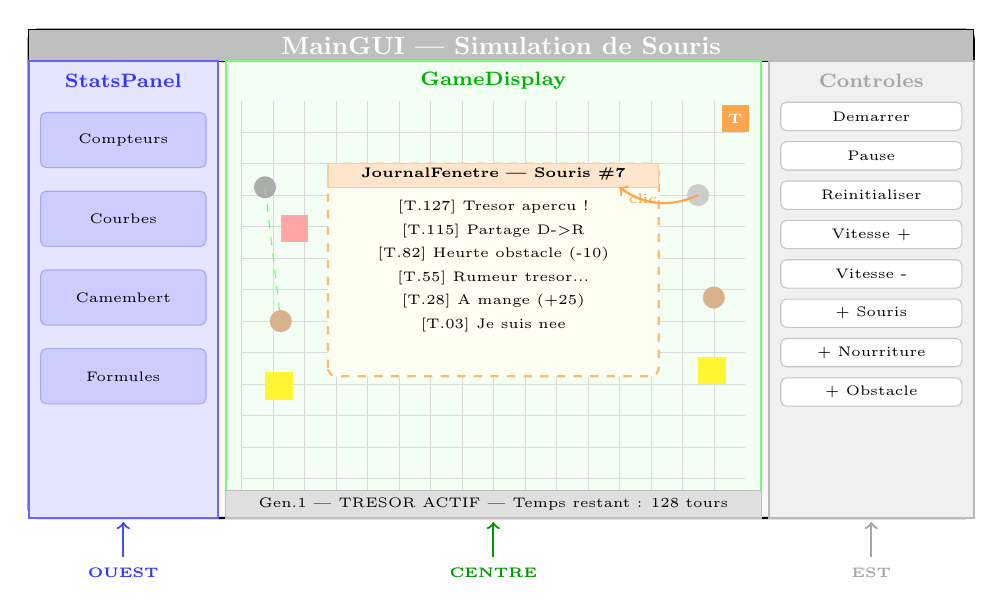
\begin{tikzpicture}[font=\scriptsize]
  \draw[fill=gray!5, draw=black, thick, rounded corners=3pt]
      (0,0) rectangle (12,6.2);
  \draw[fill=black!25, draw=black]
      (0,5.8) rectangle (12,6.2);
  \node[font=\small\bfseries, color=white] at (6,6.0)
      {MainGUI --- Simulation de Souris};
  \draw[fill=blue!10, draw=blue!60, thick]
      (0,0) rectangle (2.4,5.8);
  \node[font=\scriptsize\bfseries, color=blue!80] at (1.2,5.55) {StatsPanel};
  \foreach \y/\txt in {4.8/Compteurs,3.8/Courbes,2.8/Camembert,1.8/Formules}{
    \draw[fill=blue!20, draw=blue!35, rounded corners=2pt]
        (0.15,\y-0.35) rectangle (2.25,\y+0.35);
    \node[font=\tiny] at (1.2,\y) {\txt};
  }
  \draw[fill=green!5, draw=green!55, thick]
      (2.5,0) rectangle (9.3,5.8);
  \node[font=\scriptsize\bfseries, color=green!70!black] at (5.9,5.55) {GameDisplay};
  \foreach \x in {2.7,3.1,...,9.1}
      \draw[gray!30, very thin] (\x,0.35) -- (\x,5.3);
  \foreach \y in {0.5,0.9,...,5.2}
      \draw[gray!30, very thin] (2.7,\y) -- (9.1,\y);
  \fill[gray!65]  (3.0,4.2) circle (0.14);
  \fill[brown!60] (3.2,2.5) circle (0.14);
  \fill[gray!40]  (8.5,4.1) circle (0.14);
  \fill[brown!60] (8.7,2.8) circle (0.14);
  \fill[yellow!80] (3.0,1.5) rectangle (3.35,1.85);
  \fill[yellow!80] (8.5,1.7) rectangle (8.85,2.05);
  \fill[red!35]    (3.2,3.5) rectangle (3.55,3.85);
  \fill[orange!70] (8.8,4.9) rectangle (9.15,5.25);
  \node[font=\tiny\bfseries, color=white] at (8.97,5.07) {T};
  \draw[green!60, dashed, thin] (3.0,4.2) -- (3.2,2.5);
  \draw[fill=gray!25, draw=gray!50]
      (2.5,0) rectangle (9.3,0.35);
  \node[font=\tiny] at (5.9,0.17)
      {Gen.1 --- TRESOR ACTIF --- Temps restant : 128 tours};
  \draw[fill=yellow!5, draw=orange!55, thick, dashed, rounded corners=3pt]
      (3.8,1.8) rectangle (8.0,4.5);
  \draw[fill=orange!20, draw=orange!40]
      (3.8,4.2) rectangle (8.0,4.5);
  \node[font=\tiny\bfseries] at (5.9,4.37) {JournalFenetre --- Souris \#7};
  \node[font=\tiny] at (5.9,3.95) {[T.127] Tresor apercu !};
  \node[font=\tiny] at (5.9,3.65) {[T.115] Partage D->R};
  \node[font=\tiny] at (5.9,3.35) {[T.82] Heurte obstacle (-10)};
  \node[font=\tiny] at (5.9,3.05) {[T.55] Rumeur tresor...};
  \node[font=\tiny] at (5.9,2.75) {[T.28] A mange (+25)};
  \node[font=\tiny] at (5.9,2.45) {[T.03] Je suis nee};
  \draw[->, thick, orange!70] (8.5,4.1) to[bend left=30] (7.5,4.2);
  \node[font=\tiny, color=orange!80] at (7.8,4.05) {clic};
  \draw[fill=gray!12, draw=gray!55, thick]
      (9.4,0) rectangle (12,5.8);
  \node[font=\scriptsize\bfseries, color=gray!70] at (10.7,5.55) {Controles};
  \foreach \y/\lbl in {
      5.1/Demarrer,4.6/Pause,4.1/Reinitialiser,
      3.6/{Vitesse +},3.1/{Vitesse -},
      2.6/{+ Souris},2.1/{+ Nourriture},1.6/{+ Obstacle}}{
    \draw[fill=white, draw=gray!45, rounded corners=2pt]
        (9.55,\y-0.18) rectangle (11.85,\y+0.18);
    \node[font=\tiny] at (10.7,\y) {\lbl};
  }
  \draw[<-, blue!70, thick] (1.2,-0.05) -- (1.2,-0.5)
      node[below, font=\tiny\bfseries, color=blue!80] {OUEST};
  \draw[<-, green!60!black, thick] (5.9,-0.05) -- (5.9,-0.5)
      node[below, font=\tiny\bfseries] {CENTRE};
  \draw[<-, gray!70, thick] (10.7,-0.05) -- (10.7,-0.5)
      node[below, font=\tiny\bfseries] {EST};
\end{tikzpicture}
\end{center}
\caption{Vue globale de la fenetre principale --- MainGUI (BorderLayout)}
\label{fig:ihm_global}
\end{figure}

\paragraph{} La fenêtre principale \texttt{MainGUI} est organisée selon un \texttt{BorderLayout} en trois zones fixes. À l'\textbf{ouest}, le \texttt{StatsPanel} affiche les statistiques dynamiques de la simulation. Au \textbf{centre}, le \texttt{GameDisplay} affiche la grille animée. À l'\textbf{est}, le panneau de contrôle contient huit boutons d'action. Une fenêtre contextuelle non-modale, \texttt{JournalFenetre}, s'ouvre au clic sur une souris.

\subsubsection{Detail : le StatsPanel}

\paragraph{} Le \texttt{StatsPanel} est dessiné entièrement en Java2D, sans librairie externe. Il contient cinq blocs mis à jour à chaque appel de \texttt{nextRound()} : les compteurs rapides, la courbe de population et de nourriture, la courbe d'énergie moyenne, le camembert des types d'interactions et les formules de probabilité avec le score de colonisation courant.

\begin{figure}[h!]
\begin{center}
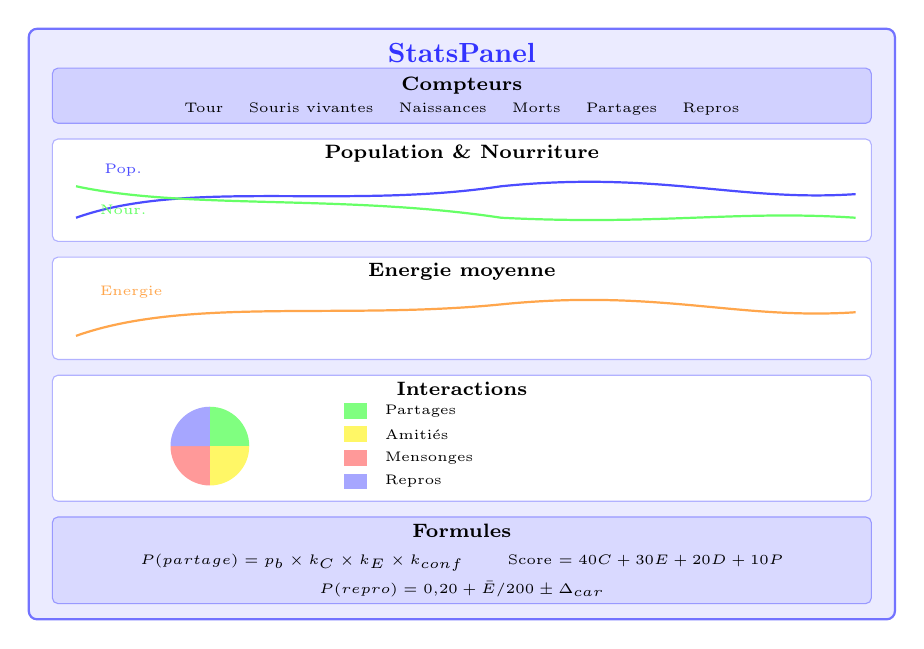
\begin{tikzpicture}[font=\scriptsize]
  \draw[fill=blue!8, draw=blue!55, thick, rounded corners=3pt]
      (0,0) rectangle (11,7.5);
  \node[font=\normalsize\bfseries, color=blue!80] at (5.5,7.2) {StatsPanel};
  \draw[fill=blue!18, draw=blue!40, rounded corners=2pt]
      (0.3,6.3) rectangle (10.7,7.0);
  \node[font=\scriptsize\bfseries] at (5.5,6.78) {Compteurs};
  \node[font=\tiny] at (5.5,6.48)
      {Tour \quad Souris vivantes \quad Naissances \quad Morts \quad Partages \quad Repros};
  \draw[fill=white, draw=blue!30, rounded corners=2pt]
      (0.3,4.8) rectangle (10.7,6.1);
  \node[font=\scriptsize\bfseries] at (5.5,5.92) {Population \& Nourriture};
  \draw[blue!70, thick]
      (0.6,5.1) .. controls (2,5.6) and (4,5.2) ..
      (6,5.5) .. controls (8,5.7) and (9,5.3) .. (10.5,5.4);
  \draw[green!60, thick]
      (0.6,5.5) .. controls (2,5.2) and (4,5.4) ..
      (6,5.1) .. controls (8,5.0) and (9,5.2) .. (10.5,5.1);
  \node[font=\tiny, color=blue!70] at (1.2,5.7) {Pop.};
  \node[font=\tiny, color=green!60] at (1.2,5.2) {Nour.};
  \draw[fill=white, draw=blue!30, rounded corners=2pt]
      (0.3,3.3) rectangle (10.7,4.6);
  \node[font=\scriptsize\bfseries] at (5.5,4.42) {Energie moyenne};
  \draw[orange!70, thick]
      (0.6,3.6) .. controls (2,4.1) and (4,3.8) ..
      (6,4.0) .. controls (8,4.2) and (9,3.8) .. (10.5,3.9);
  \node[font=\tiny, color=orange!70] at (1.3,4.15) {Energie};
  \draw[fill=white, draw=blue!30, rounded corners=2pt]
      (0.3,1.5) rectangle (10.7,3.1);
  \node[font=\scriptsize\bfseries] at (5.5,2.93) {Interactions};
  \fill[green!50]  (2.3,2.2) -- (2.3,2.7) arc(90:0:0.5) -- cycle;
  \fill[yellow!60] (2.3,2.2) -- (2.8,2.2) arc(0:-90:0.5) -- cycle;
  \fill[red!40]    (2.3,2.2) -- (2.3,1.7) arc(270:180:0.5) -- cycle;
  \fill[blue!35]   (2.3,2.2) -- (1.8,2.2) arc(180:90:0.5) -- cycle;
  \fill[green!50]  (4.0,2.55) rectangle (4.3,2.75);
  \node[font=\tiny, anchor=west] at (4.4,2.65) {Partages};
  \fill[yellow!60] (4.0,2.25) rectangle (4.3,2.45);
  \node[font=\tiny, anchor=west] at (4.4,2.35) {Amitiés};
  \fill[red!40]    (4.0,1.95) rectangle (4.3,2.15);
  \node[font=\tiny, anchor=west] at (4.4,2.05) {Mensonges};
  \fill[blue!35]   (4.0,1.65) rectangle (4.3,1.85);
  \node[font=\tiny, anchor=west] at (4.4,1.75) {Repros};
  \draw[fill=blue!15, draw=blue!40, rounded corners=2pt]
      (0.3,0.2) rectangle (10.7,1.3);
  \node[font=\scriptsize\bfseries] at (5.5,1.12) {Formules};
  \node[font=\tiny] at (5.5,0.72)
      {$P(\text{partage}) = p_b \times k_C \times k_E \times k_{conf}$
       \qquad Score $= 40C + 30E + 20D + 10P$};
  \node[font=\tiny] at (5.5,0.38)
      {$P(\text{repro}) = 0{,}20 + \bar{E}/200 \pm \Delta_{car}$};
\end{tikzpicture}
\end{center}
\caption{Detail du StatsPanel --- 5 blocs mis a jour a chaque tour}
\label{fig:statspanel}
\end{figure}

\bigskip

\subsubsection{Detail : le GameDisplay}

\begin{figure}[h!]
\begin{center}
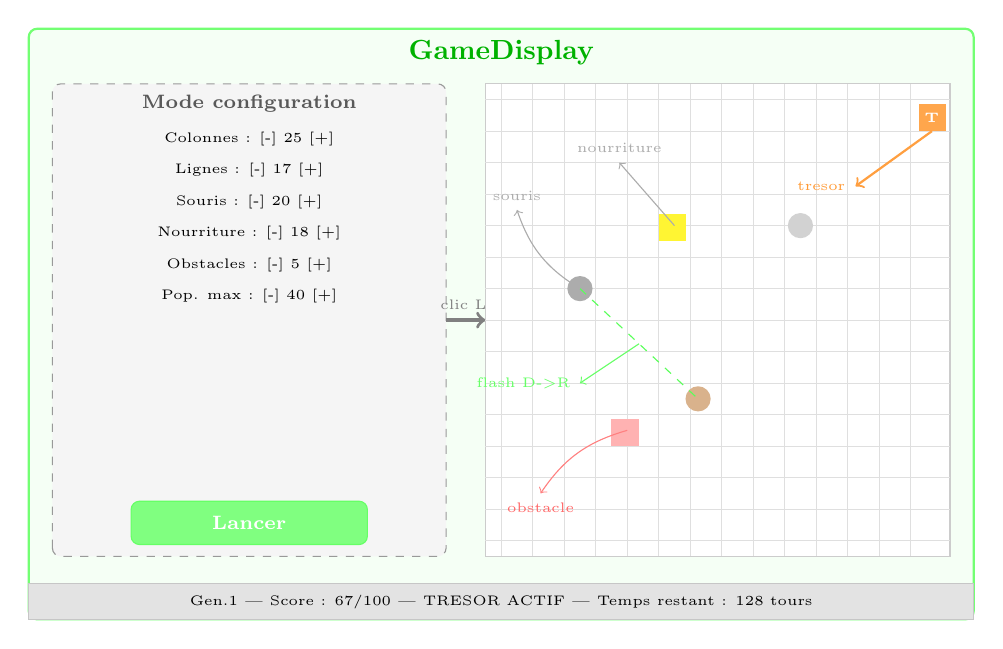
\begin{tikzpicture}[font=\scriptsize]
  \draw[fill=green!4, draw=green!55, thick, rounded corners=3pt]
      (0,0) rectangle (12,7.5);
  \node[font=\normalsize\bfseries, color=green!70!black] at (6,7.2) {GameDisplay};
  \draw[fill=gray!8, draw=black!40, dashed, rounded corners=3pt]
      (0.3,0.8) rectangle (5.3,6.8);
  \node[font=\scriptsize\bfseries, color=black!65] at (2.8,6.55)
      {Mode configuration};
  \foreach \y/\lbl in {
      6.1/{Colonnes : [-] 25 [+]},5.7/{Lignes : [-] 17 [+]},
      5.3/{Souris : [-] 20 [+]},4.9/{Nourriture : [-] 18 [+]},
      4.5/{Obstacles : [-] 5 [+]},4.1/{Pop. max : [-] 40 [+]}}{
    \node[font=\tiny] at (2.8,\y) {\lbl};
  }
  \draw[fill=green!50, draw=green!60, rounded corners=3pt]
      (1.3,0.95) rectangle (4.3,1.5);
  \node[font=\scriptsize\bfseries, color=white] at (2.8,1.22) {Lancer};
  \draw[->, very thick, black!50] (5.3,3.8) -- (5.8,3.8)
      node[above, font=\tiny] {clic Lancer};
  \draw[fill=white, draw=gray!40]
      (5.8,0.8) rectangle (11.7,6.8);
  \foreach \x in {6.0,6.4,...,11.5}
      \draw[gray!25, very thin] (\x,0.8) -- (\x,6.8);
  \foreach \y in {1.0,1.4,...,6.6}
      \draw[gray!25, very thin] (5.8,\y) -- (11.7,\y);
  \fill[gray!65]  (7.0,4.2) circle (0.16);
  \fill[brown!60] (8.5,2.8) circle (0.16);
  \fill[gray!35]  (9.8,5.0) circle (0.16);
  \fill[yellow!80] (8.0,4.8) rectangle (8.35,5.15);
  \fill[red!30]    (7.4,2.2) rectangle (7.75,2.55);
  \fill[orange!70] (11.3,6.2) rectangle (11.65,6.55);
  \node[font=\tiny\bfseries, color=white] at (11.47,6.37) {T};
  \draw[green!65, dashed, thin] (7.0,4.2) -- (8.5,2.8);
  \draw[->, gray!65] (7.0,4.2) to[bend left=20] (6.2,5.2)
      node[above, font=\tiny] {souris};
  \draw[->, gray!65] (8.2,5.0) -- (7.5,5.8)
      node[above, font=\tiny] {nourriture};
  \draw[->, red!50] (7.6,2.4) to[bend right=20] (6.5,1.6)
      node[below, font=\tiny, color=red!60] {obstacle};
  \draw[->, orange!75, thick] (11.47,6.2) -- (10.5,5.5)
      node[left, font=\tiny, color=orange!80] {tresor};
  \draw[->, green!60] (7.75,3.5) -- (7.0,3.0)
      node[left, font=\tiny, color=green!60] {flash D->R};
  \draw[fill=gray!22, draw=gray!45] (0,0) rectangle (12,0.45);
  \node[font=\tiny] at (6,0.22)
      {Gen.1 --- Score : 67/100 --- TRESOR ACTIF --- Temps restant : 128 tours};
\end{tikzpicture}
\end{center}
\caption{Detail du GameDisplay (overlay config. a gauche, grille de simulation a droite)}
\label{fig:gamedisplay}
\end{figure}

\paragraph{} Le \texttt{GameDisplay} a deux modes de fonctionnement. Au démarrage, il affiche l'overlay de configuration permettant de régler les paramètres avec des boutons $[-]$/$[+]$. Après le clic sur ``Lancer'', il affiche la grille de simulation en temps réel avec les souris, nourritures, obstacles, flashes et le trésor. La barre d'état en bas affiche le tour courant, le score et l'état du trésor.

\bigskip

\subsubsection{Detail : la JournalFenetre}

\paragraph{} La \texttt{JournalFenetre} est une \texttt{JDialog} non-modale qui s'ouvre lorsque l'utilisateur clique sur une souris dans la grille. Elle est implémentée comme un Singleton : une seule instance existe, et son contenu se met à jour selon la souris cliquée. Elle affiche l'identité complète de la souris en en-tête, puis son journal intime en ordre anti-chronologique avec un code couleur par type d'événement.

\begin{figure}[h!]
\begin{center}
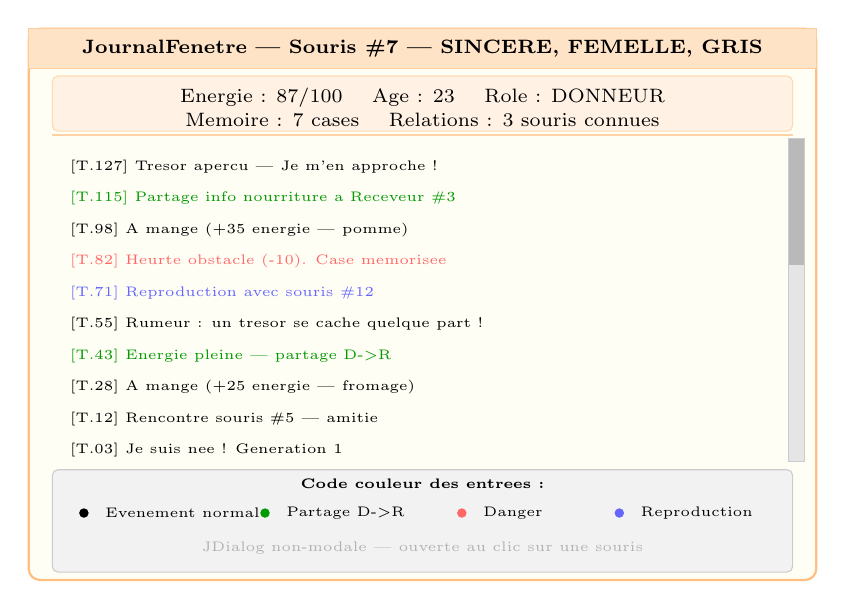
\begin{tikzpicture}[font=\scriptsize]
  \draw[fill=yellow!4, draw=orange!50, thick, rounded corners=4pt]
      (0,0) rectangle (10,7.0);
  \draw[fill=orange!22, draw=orange!40]
      (0,6.5) rectangle (10,7.0);
  \node[font=\scriptsize\bfseries] at (5,6.75)
      {JournalFenetre --- Souris \#7 --- SINCERE, FEMELLE, GRIS};
  \draw[fill=orange!10, draw=orange!30, rounded corners=2pt]
      (0.3,5.7) rectangle (9.7,6.4);
  \node[font=\scriptsize] at (5,6.12)
      {Energie : 87/100 \quad Age : 23 \quad Role : DONNEUR};
  \node[font=\scriptsize] at (5,5.85)
      {Memoire : 7 cases \quad Relations : 3 souris connues};
  \draw[orange!35, thick] (0.3,5.65) -- (9.7,5.65);
  \foreach \y/\col/\txt in {
      5.25/black/{[T.127] Tresor apercu --- Je m'en approche !},
      4.85/green!60!black/{[T.115] Partage info nourriture a Receveur \#3},
      4.45/black/{[T.98]  A mange (+35 energie --- pomme)},
      4.05/red!60/{[T.82]  Heurte obstacle (-10). Case memorisee},
      3.65/blue!60/{[T.71]  Reproduction avec souris \#12},
      3.25/black/{[T.55]  Rumeur : un tresor se cache quelque part !},
      2.85/green!60!black/{[T.43]  Energie pleine --- partage D->R},
      2.45/black/{[T.28]  A mange (+25 energie --- fromage)},
      2.05/black/{[T.12]  Rencontre souris \#5 --- amitie},
      1.65/black/{[T.03]  Je suis nee ! Generation 1}}{
    \node[font=\tiny, color=\col, anchor=west] at (0.4,\y) {\txt};
  }
  \draw[fill=gray!20, draw=gray!40] (9.65,1.5) rectangle (9.85,5.6);
  \fill[gray!55] (9.65,4.0) rectangle (9.85,5.6);
  \draw[fill=gray!10, draw=gray!40, rounded corners=2pt]
      (0.3,0.1) rectangle (9.7,1.4);
  \node[font=\tiny\bfseries] at (5,1.22) {Code couleur des entrees :};
  \fill[black]          (0.7,0.85) circle (0.06);
  \node[font=\tiny, anchor=west] at (0.85,0.85) {Evenement normal};
  \fill[green!60!black] (3.0,0.85) circle (0.06);
  \node[font=\tiny, anchor=west] at (3.15,0.85) {Partage D->R};
  \fill[red!60]         (5.5,0.85) circle (0.06);
  \node[font=\tiny, anchor=west] at (5.65,0.85) {Danger};
  \fill[blue!60]        (7.5,0.85) circle (0.06);
  \node[font=\tiny, anchor=west] at (7.65,0.85) {Reproduction};
  \node[font=\tiny, color=gray!60] at (5,0.4)
      {JDialog non-modale --- ouverte au clic sur une souris};
\end{tikzpicture}
\end{center}
\caption{Detail de la JournalFenetre (fenetre contextuelle par souris)}
\label{fig:journal}
\end{figure}
\subsection{Journalisation avec Log4j}

\paragraph{} La journalisation est assurée par le framework \textbf{Log4j 1.2.17}, fourni par M. Liu dans le cadre du TD 6. La classe \texttt{LoggerUtility} (identique à \textit{tree\_v3}) offre deux modes de sortie : texte (pour la console et le fichier \texttt{log/souris-log.txt}) et HTML (pour le fichier \texttt{log/souris-log.html}).

\paragraph{} La différence avec la version originale de \textit{tree\_v3} réside dans le chargement des fichiers de configuration. Dans notre version, les \texttt{.properties} sont chargés via \texttt{getResourceAsStream} depuis le classpath plutôt que par un chemin fichier relatif. Cela garantit que les logs fonctionnent correctement quelle que soit la façon dont Eclipse lance le programme.

\begin{lstlisting}[caption={Chargement des properties Log4j via le classpath}]
public static Logger getLogger(Class<?> logClass,
                               String logFileType) {
    try {
        String configFile = logFileType.equals("html")
            ? "log/log4j-html.properties"
            : "log/log4j-text.properties";
        InputStream is = LoggerUtility.class
            .getClassLoader()
            .getResourceAsStream(configFile);
        if (is != null) {
            Properties props = new Properties();
            props.load(is);
            PropertyConfigurator.configure(props);
        }
    } catch (Exception e) {
        System.err.println("Log4j config error: "
            + e.getMessage());
    }
    return Logger.getLogger(logClass.getName());
}
\end{lstlisting}

\paragraph{} Les événements loggés couvrent l'ensemble du cycle de vie de la simulation : création des souris, déplacements significatifs, interactions D$\rightarrow$R, reproductions, morts, apparition du trésor, conditions de fin et score final.
